\begin{example}
    Consider the following network where we want to check the property
    that $d$ is being blacklisted:
    \begin{center}
        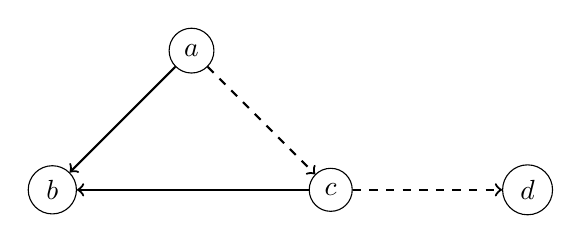
\begin{tikzpicture}[node distance={25mm},
                main/.style = {draw, circle},
                s/.style = {->,thick},
                d/.style = {->,thick,dashed} ]
            \node[main] (b) {$b$};
            \node[main] (a) [above right of=b] {$a$};
            \node[main] (c) [below right of=a] {$c$};
            \node[main] (d) [right of=c] {$d$};
            \draw[s] (a) -- (b);
            \draw[d] (a) -- (c);
            \draw[s] (c) -- (b);
            \draw[d] (c) -- (d);
        \end{tikzpicture}
    \end{center}
    We define this network using the following DyNetKAT term:
    \begin{align*}
        S_{xy}  & = sw = x \cdot sw \la y            \\
        P       & = u!S_{ac}                         \\
        Q       & = u!S_{cd}                         \\
        N_{x,y} & = (S_x+S_y)^* \oplus u?x';N_{x',y}
        \oplus u?y';N_{x,y'}                         \\
        SDN     & = \delta_{\mathcal{L}} (N_{ab,cb}
        \parallel P \parallel Q)
    \end{align*}
    Where $\mathcal{L} = \s{u!S_{ac},u?S_{ac},u!S_{cd},u?S_{cd}}$.
    We may rewrite the terms as follows:
    \begin{align*}
        N_{ab,cb} & = (S_{ab} + S_{cb})^* \oplus u?S_{ac};N_{ac,cb}
        \oplus u?S_{cd};N_{ab,cd}                                   \\
        N_{ac,cb} & = (S_{ac}+S_{cb})^* \oplus u?S_{cd};N_{ac,cd}   \\
        N_{ab,cd} & = (S_{ab}+S_{cd})^* \oplus u?S_{ac};N_{ac,cd}   \\
        N_{ac,cd} & = (S_{ac}+S_{cd})^*
    \end{align*}
    Assume that we are considering this network under the situation where
    a single packet arrived at $a$.
    Thus we can assume consider a packet $\sigma$ arrived where
    $\sigma(sw) = a$.
    Under this condition, we can replace the NetKAT terms with
    packet forwarding actions of the form $(\sigma, \sigma')$.
    We use $xy$ to denote an action of the form $(\sigma,\sigma')$
    where $\sigma(sw) = x$ and $\sigma'(sw) = y$.
    For a DyNetKAT term $T$, we use $T^a$ to denote the term where
    we have replaced all NetKAT policies with packet forwarding actions.
    Furthermore, we rename actions
    $u?S_{ac},u!S_{ac},u?S_{cd},u!S_{cd}$ to $u_a,u_a',u_c,u_c'$ respectively,
    so we can derive the following terms:
    \begin{align*}
        SDN^a       & = \delta_{\mathcal{L}}
        ( N^a_{ab,cb} \parallel P \parallel Q)               \\
        P           & = u_a'                                \\
        Q           & = u_c'                                \\
        N^a_{ab,cb} & = ab \oplus u_a;N^a_{ac,cb}
        \oplus u_c;N^a_{ab,cd}                              \\
        N^a_{ac,cb} & = ac \oplus ab \oplus u_c;N^a_{ac,cd} \\
        N^a_{ab,cd} & = ab \oplus u_a;N^a_{ac,cd}           \\
        N^a_{ac,cd} & = ac \oplus ad
    \end{align*}
    Let we use $p,q$ for the actions $rcfg(u_a,u_a'),rcfg(u_c,u_c')$
    respectively so we can derive the following LTS for $SDN^u$:
    \begin{center}
        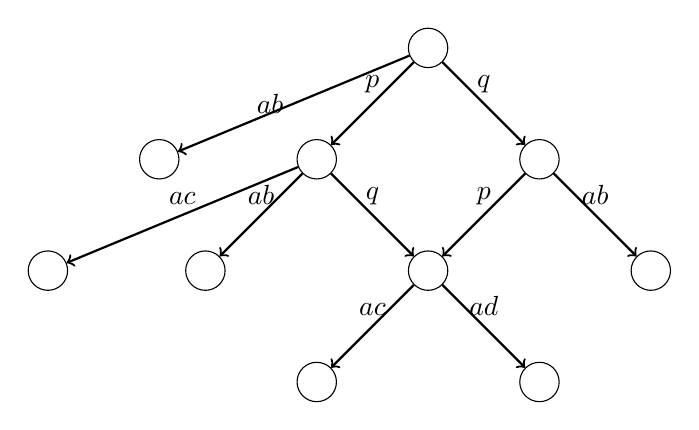
\begin{tikzpicture}[node distance={20mm},
                main/.style = {draw, circle,minimum width=5mm},
                s/.style = {->,thick}]
            \node[main] (s1) {};
            \node[main] (s3) [below left of=s1] {};
            \node[main] (s4) [below right of=s1] {};
            \node[main] (s2) [left of=s3] {};
            \node[main] (s6) [below left of=s3] {};
            \node[main] (s7) [below right of=s3] {};
            \node[main] (s5) [left of=s6] {};
            \node[main] (s8) [below right of=s4] {};
            \node[main] (s9) [below left of=s7] {};
            \node[main] (s10) [below right of=s7] {};
            \draw[s] (s1) -- node[left]{$ab$} (s2);
            \draw[s] (s1) -- node[above]{$p$}(s3);
            \draw[s] (s1) -- node[above]{$q$}(s4);
            \draw[s] (s3) -- node[above]{$ac$}(s5);
            \draw[s] (s3) -- node[above]{$ab$}(s6);
            \draw[s] (s3) -- node[above]{$q$}(s7);
            \draw[s] (s4) -- node[above]{$p$}(s7);
            \draw[s] (s4) -- node[above]{$ab$}(s8);
            \draw[s] (s7) -- node[above]{$ac$}(s9);
            \draw[s] (s7) -- node[above]{$ad$}(s10);
        \end{tikzpicture}
        \begin{center}
            \begin{tikzpicture}[u/.style ={ultra thick}]
                \crd{0}{0}{$\emptyset$}
                \crd[left]{-1}{-1}{$\s{p_1}$}
                \crd[right]{1}{-1}{$\s{q_2}$}
                \crd[above]{-3}{-1}{$\s{ab_1}$}
                \crd[right]{-1}{-2}{$\s{p_1,q_1}$}
                \crd[below]{-2}{-2}{$\s{p_1,ab_2}$}
                \crd[left]{-3}{-2}{$\s{p_1,ac_1}$}
                \crd[below]{-1}{-3}{$\s{p_1,q_1,ad_1}$}
                \crd[left]{-2}{-3}{$\s{p_1,q_1,ac_2}$}
                \crd[above]{1}{-2}{$\s{p_2,q_2}$}
                \crd[right]{2}{-2}{$\s{q_2,ab_2}$}
                \crd[below]{1}{-3}{$\s{p_2,q_2,ad_2}$}
                \crd[right]{2}{-3}{$\s{p_2,q_2,ac_3}$}
                \draw [u] (0,0) -- (-1,-1);
                \draw [u] (0,0) -- (1,-1);
                \draw [u] (0,0) -- (-3,-1);
                \draw [u] (-1,-1) -- (-1,-2);
                \draw [u] (-1,-1) -- (-2,-2);
                \draw [u] (-1,-1) -- (-3,-2);
                \draw [u] (-1,-2) -- (-1,-3);
                \draw [u] (-1,-2) -- (-2,-3);
                \draw [u] (1,-1) -- (1,-2);
                \draw [u] (1,-1) -- (2,-2);
                \draw [u] (1,-2) -- (1,-3);
                \draw [u] (1,-2) -- (2,-3);
            \end{tikzpicture}
        \end{center}
    \end{center}
    We may define the event structure $\mathrm{E} = (E,\#,\vdash,L,l)$ for $SDN^u$
    where we have:
    \begin{align*}
         & E = \s{ab_1,ab_2,ab_3,ac_1,ac_2,ad_1,ad_2,p_1,p_2,q_1,q_2}              \\
         & l(ab_1) = ab, l(ab_2) = ab, l(ab_3) = ab, l(ac_1) = ac, l(ac_2) = ac    \\
         & l(ad_1) = ad,l(ad_2)=ad, l(p_1) = p, l(p_2) = p, l(q_1) = q, l(q_2) = q
    \end{align*}
    Enabling relation the least one that satisfies:
    \begin{align*}
         & \e \vdash ab_1, \e \vdash p_1, \e \vdash q_2,
        \s{p_1} \vdash ac_1, \s{p_1} \vdash ab_2, \s{p_1} \vdash q_1,
        \s{q_1} \vdash p_2, \s{q_1} \vdash ab_3              \\
         & \s{p_1,q_1} \vdash ac_2, \s{p_1,q_1} \vdash ad_1,
        \s{p_2,q_2} \vdash ac_2, \s{p_2,q_2} \vdash ad_2
    \end{align*}
    Here we have considered the switch $d$ as a blacklist, thus we can define the
    safety property $P$ as follows:
    \begin{align*}
        P = \s{s|\forall e \in s. l(e) = (\sigma,\sigma')\wedge \sigma'(sw) \neq d}
    \end{align*}
    Let $\mathcal{C} = \mathcal{P}(E) - P$.
    $C$ contains subsets of $E$ that contains either $ad_1$ or $ad_2$.
    To find the cause of the $P$'s violation in $\mathrm{E}$, we construct the
    causal model $M = \mathfrak{M}(\mathrm{E},\mathcal{C})$.
    Assume that we wish to declare $C(p_1,q_1) = \F$ as a cause using the witness
    $(C(p_2,q_2),\T,\T)$.
    Since $\s{p_1,q_1,ad_1}$ is a configuration of $\mathrm{E}$ thus
    $AC1$ is satisfied.
    Now assume that we set both $C(p_1,q_1)$ and $C(p_2,q_2)$ to true.
    Since we have $\s{p_1,q_1} \vdash_{min} ad_1$ and
    $\s{p_2,q_2} \vdash_{min} ad_2$ and also $p_1\#q_1$ and $p_2\#q_2$ in $ES$,
    thus neither $\s{p_1,q_1,ad_1}$ nor $\s{p_2,q_2,ad_2}$ are not
    configurations of $ES$ so AC2(a) is satisfied.
    Now assume that we only set $C(p_2,q_2)$ to true.
    In this case $\s{p_1,q_1,ad_1}$ is a configuration of $ES$ even if reset any
    variable to its original value in the actual context.
    So finally we can conclude that $C(p_1,q_1) = \F$ is an actual cause of the
    violation of $P$ in $E$.
\end{example}